\documentclass[conference]{IEEEtran}
\IEEEoverridecommandlockouts
\usepackage{cite}
\usepackage{amsmath,amssymb,amsfonts}
\usepackage{graphicx}
\usepackage{textcomp}
\usepackage{xcolor}
\usepackage{booktabs}
\usepackage{tikz}
\usepackage{pgfplots}
\pgfplotsset{compat=1.17}
\usetikzlibrary{positioning,arrows.meta,fit,backgrounds}
\usepackage{hyperref}
\usepackage{url}

\def\BibTeX{{\rm B\kern-.05em{\sc i\kern-.025em b}\kern-.08em
    T\kern-.1667em\lower.7ex\hbox{E}\kern-.125emX}}

\begin{document}

\title{ARGUS: A Deterministic Scene-Graph Compiler with\\Vision-Guided Symbolic Repair for Text-to-3D Asset Synthesis}

\author{
\IEEEauthorblockN{Darpan Dahal}
\IEEEauthorblockA{
Department of Computer Engineering \\
Sikkim Institute of Science and Technology, Sikkim University \\
Sikkim, India \\
darpandahal111@gmail.com}
}

\maketitle

\begin{abstract}
Text-to-3D systems commonly trade off visual quality, structural editability, and production reliability. Neural methods can produce detailed geometry but do not necessarily expose named, independently editable parts. LLM-based code-generation systems expose a programmatic representation, but couple spatial planning to low-level scene construction. This paper presents ARGUS, a systems pipeline that separates those responsibilities. An LLM first writes a compact build plan containing named parts, primitive types, dimensions, materials, and attachments. A rule-based compiler then maps the plan to Blender geometry using a fixed library of construction routines. When a rendered result does not satisfy the plan, a vision-language model proposes bounded edits to the plan; full script generation remains a fallback path. The compiler and export pipeline also provide artifact-level measurements of topology, materials, and polygon count. In a pilot run of 15 prompts sampled from a 30-prompt hard-surface benchmark, all prompts produced an exported artifact, 13/15 artifacts were classified as clean by the implemented topology checker, 13/15 contained at least one glTF material with a base-color texture, and the mean model-judged visual score was 6.67/10. We use a topology/material-aware effective score only as a candidate-selection heuristic; it is not presented as a validated perceptual metric. The pilot includes no external baseline, ablation study, or human evaluation, so the results establish system behavior and reproducibility targets rather than comparative superiority.
\end{abstract}

\begin{IEEEkeywords}
text-to-3D generation, program synthesis, large language models, procedural modeling, vision-language feedback, mesh topology checking
\end{IEEEkeywords}

\section{Introduction}

Text-to-3D generation is increasingly used to create assets for interactive applications, but generated assets must satisfy constraints that are not captured by appearance alone: parts should remain identifiable, geometry should be exportable, materials should survive the export path, and failures should be repairable. Existing approaches occupy different points in this design space.

\textbf{Neural generative methods} include score-distillation approaches, which optimize a neural radiance field against a 2D diffusion model \cite{poole2023dreamfusion,lin2023magic3d,chen2023fantasia3d}, and feed-forward models, which map an image or text straight to a 3D shape in one pass \cite{jun2023shape,tochilkin2024triposr,xiang2024trellis}. These methods can produce visually compelling results, but their output representation does not necessarily expose the semantic part structure needed for direct editing. Geometry quality and part-level editability also depend on the particular model and export pipeline, so they should be measured rather than assumed.

\textbf{LLM-as-code-writer systems} \cite{lu2025ll3m,yang2024scenecraft} instead have a language model write real Blender Python code by hand. This keeps the result editable as a program, but it couples scene-level spatial decisions to low-level API calls and syntax. A local geometric error can therefore require a broad script rewrite. ARGUS treats this coupling as a design problem and evaluates whether a structured intermediate representation makes repair more localized.

ARGUS splits these two jobs apart instead of asking one bigger model to do both well. First, an LLM writes a \emph{build plan}: a list of named parts, where each part has a basic shape picked from a small, fixed list (box, cylinder, sphere, lathe profile, tube, wheel, ring, and a few others), a size, a position, and a note on which part it connects to. This plan is small, easy-to-read JSON, not code. A separate, rule-based compiler then turns the plan into a real Blender scene using a fixed set of shape-building functions that always produce clean, closed geometry, with finishing touches (edge rounding, smoothing, tapering) applied automatically from the plan instead of being hand-coded by the model for every object. When a rendered image does not match the prompt, a vision-language model is asked to suggest a short list of small changes to the \emph{plan}, not a full script rewrite: add a missing part, resize one piece, taper a part that looks too boxy. The compiler then rebuilds the object from the updated plan. Writing a full script by hand is kept only as a backup, used when a plan cannot be created or compiled at all.

This design extends an earlier version of the project, described in an unpublished undergraduate report \cite{dahal2026thesis}, in which an LLM generated the Blender script directly. The present paper studies the plan-and-compile architecture as a systems contribution and reports the current pilot measurements without attributing causal improvements to any component that has not yet been isolated experimentally.

\subsection*{Contributions}
\begin{enumerate}
\item A simple build-plan format and a rule-based compiler that turns it into 3D geometry for hard-surface objects, so the LLM only has to plan and does not also have to get geometry code right.
\item A repair loop guided by a vision-language model that edits the plan instead of rewriting code, with full script rewriting kept only as a backup.
\item A topology/material-aware candidate-selection heuristic that supplements a model-judged visual score with measurements extracted from the exported artifact.
\item A public evaluation harness containing 30 hard-surface prompts across three difficulty levels, deterministic artifact metrics, and configurable experimental conditions.
\item A documented pilot run on 15 prompts (5 per difficulty level), reported as a systems characterization rather than as a comparative benchmark.
\end{enumerate}

\section{Related Work}
\label{sec:related}

\subsection{Neural 3D Generation}
Denoising diffusion models learn to build an image by slowly removing noise from random static \cite{ho2020ddpm}. DreamFusion \cite{poole2023dreamfusion} built on this idea with a method called Score Distillation Sampling: it optimizes a neural radiance field (NeRF) using a 2D diffusion model as a guide, without needing any real 3D training data. Magic3D \cite{lin2023magic3d} and Fantasia3D \cite{chen2023fantasia3d} improved this same family for image quality and for keeping shape and appearance separate during training, with Fantasia3D representing geometry as a signed distance field trained apart from a physically based surface-appearance model. Feed-forward methods skip the slow per-prompt optimization step entirely: Point-E \cite{nichol2022pointe} and its successor Shap-E \cite{jun2023shape} generate a 3D shape in one fast pass, TripoSR \cite{tochilkin2024triposr} builds a mesh from a single picture in under half a second, TRELLIS \cite{xiang2024trellis} stores shape, texture, and material together in one learned representation, and Hunyuan3D 2.0 \cite{hunyuan3d2025} scales this same style of model up for high-resolution, textured results. Latent diffusion \cite{rombach2022ldm} and the original neural radiance field paper \cite{mildenhall2020nerf} are the foundation much of this family is built on. None of these systems produce parts you can pick out and edit separately; the output is one mesh or one neural field, and whatever real-world structure the object has (a handle, a lid, a leg) is not stored anywhere in the representation.

\subsection{Programmatic and Procedural Shape Representations}
A different line of work treats shapes as small programs instead of raw geometry. ShapeAssembly \cite{jones2020shapeassembly} defines a simple assembly language where shapes are built from box-shaped parts connected with symmetry and attachment rules, and trains a model to write programs in that language. This gives real structure and part-level editing, but it only supports boxes and needs matched program-and-shape training pairs, so it cannot work from an open-ended text prompt. Older procedural-modeling work builds structured output from hand-written rules, without any language model or generative step at all \cite{merrell2011modelsynthesis}. ARGUS's build-plan format follows the same programs-not-pixels idea, but swaps a fixed grammar and supervised training for an LLM-written, JSON-based plan, evaluated by a rule-based compiler with a wider set of shapes (including lathe-profile spins and tube sweeps, not just boxes) built for stylized props rather than only box-shaped furniture.

\subsection{LLM Code Generation for 3D Geometry}
The systems closest to ARGUS are ones where an LLM writes 3D geometry code directly. This whole idea rests on a simple fact shown by Codex \cite{chen2021codex}: a large language model trained on real code can write working programs from a plain description, which is also the technology GitHub Copilot is built on. SceneCraft \cite{yang2024scenecraft} builds Blender code for whole scenes from a layout plan and checks its own renders as it goes. LL3M \cite{lu2025ll3m} instead uses a team of LLM agents that split the work: one plans the object, one looks things up in a Blender-documentation index, and others write, debug, and visually check the resulting Python code. Its main idea is treating 3D modeling as teamwork between code-writing agents rather than one black-box step, while still writing Blender code directly instead of a higher-level plan. Both of these systems, and ARGUS's own earlier version \cite{dahal2026thesis}, put spatial reasoning and code-writing into the same step. If a render comes out wrong for any reason, the thing that needs fixing is a script, and fixing one part risks accidentally breaking another part in the same rewrite. ARGUS instead keeps code-writing as a backup only, and treats the plan, not the script, as the main thing that gets edited and repaired. A separate line of work uses LLMs for precision CAD design (sketch-and-extrude tools, boundary shapes) \cite{cadsurvey2025}; that work cares about exact measurements rather than the stylized, game-ready look this paper is aiming for, and it uses a different geometry engine entirely.

\subsection{Iterative Self-Refinement with External Feedback}
CLIP \cite{radford2021clip} showed that a single model can be trained to match images and text descriptions together, which is the basic building block behind almost every system, including ours, that asks a vision-language model to judge a picture against a written description. Self-Refine \cite{madaan2023selfrefine} showed that a language model can improve its own answer by generating feedback on itself and using that feedback to try again, without needing any outside training signal, across several text-writing tasks. Because a model judging its own or another model's output is now common, it is worth asking how much to trust that judgment: work on using an LLM as a judge \cite{zheng2023llmjudge} found that a strong model like GPT-4 can agree with human preference over 80\% of the time on open-ended questions, which is encouraging, but does not by itself guarantee a judge is reliable enough to trust blindly. That question matters directly for Section III-E below. Closer to our own repair loop is work that uses a vision-language model to look at a rendered webpage and give structured feedback that guides the next round of code \cite{visionguided2026}. ARGUS's own repair loop follows the same basic pattern, render it, get feedback, fix it, render it again, but applied to a different kind of picture (a multi-view grid of a 3D object) and, importantly, to a different kind of fix: the feedback becomes a short edit list against a structured plan whenever a plan exists, and only falls back to full-script feedback when it does not. That is a smaller, safer space of possible fixes than either of the systems above uses.

\subsection{Mesh Topology Validation}
Whether a mesh is watertight (no holes) and clean (no broken edges) is usually checked after the fact, either by casting rays through the surface or by counting bad edges, open boundaries, and broken faces directly \cite{huang2020manifoldplus}. The classic way to turn an implicit shape, like a signed distance field, into an actual mesh is the Marching Cubes algorithm \cite{lorensen1987marchingcubes}, which can still produce small mesh errors depending on how it is set up. ARGUS avoids that whole conversion step: its parts are built as clean meshes from the start, so there is no implicit-to-mesh step that could introduce errors in the first place. ARGUS still checks a similar set of numbers on its own (bad faces, broken edges, floating vertices, and separate disconnected pieces found using a union-find check over each part's bounding box) right inside the same Blender process that builds the object, with no extra render or export step needed, and, as we explain in Section III-E, it feeds that check straight back into which candidate gets picked, instead of only reporting it after the model is already finished.

\section{System Architecture}
\label{sec:arch}

\begin{figure}[t]
\centering
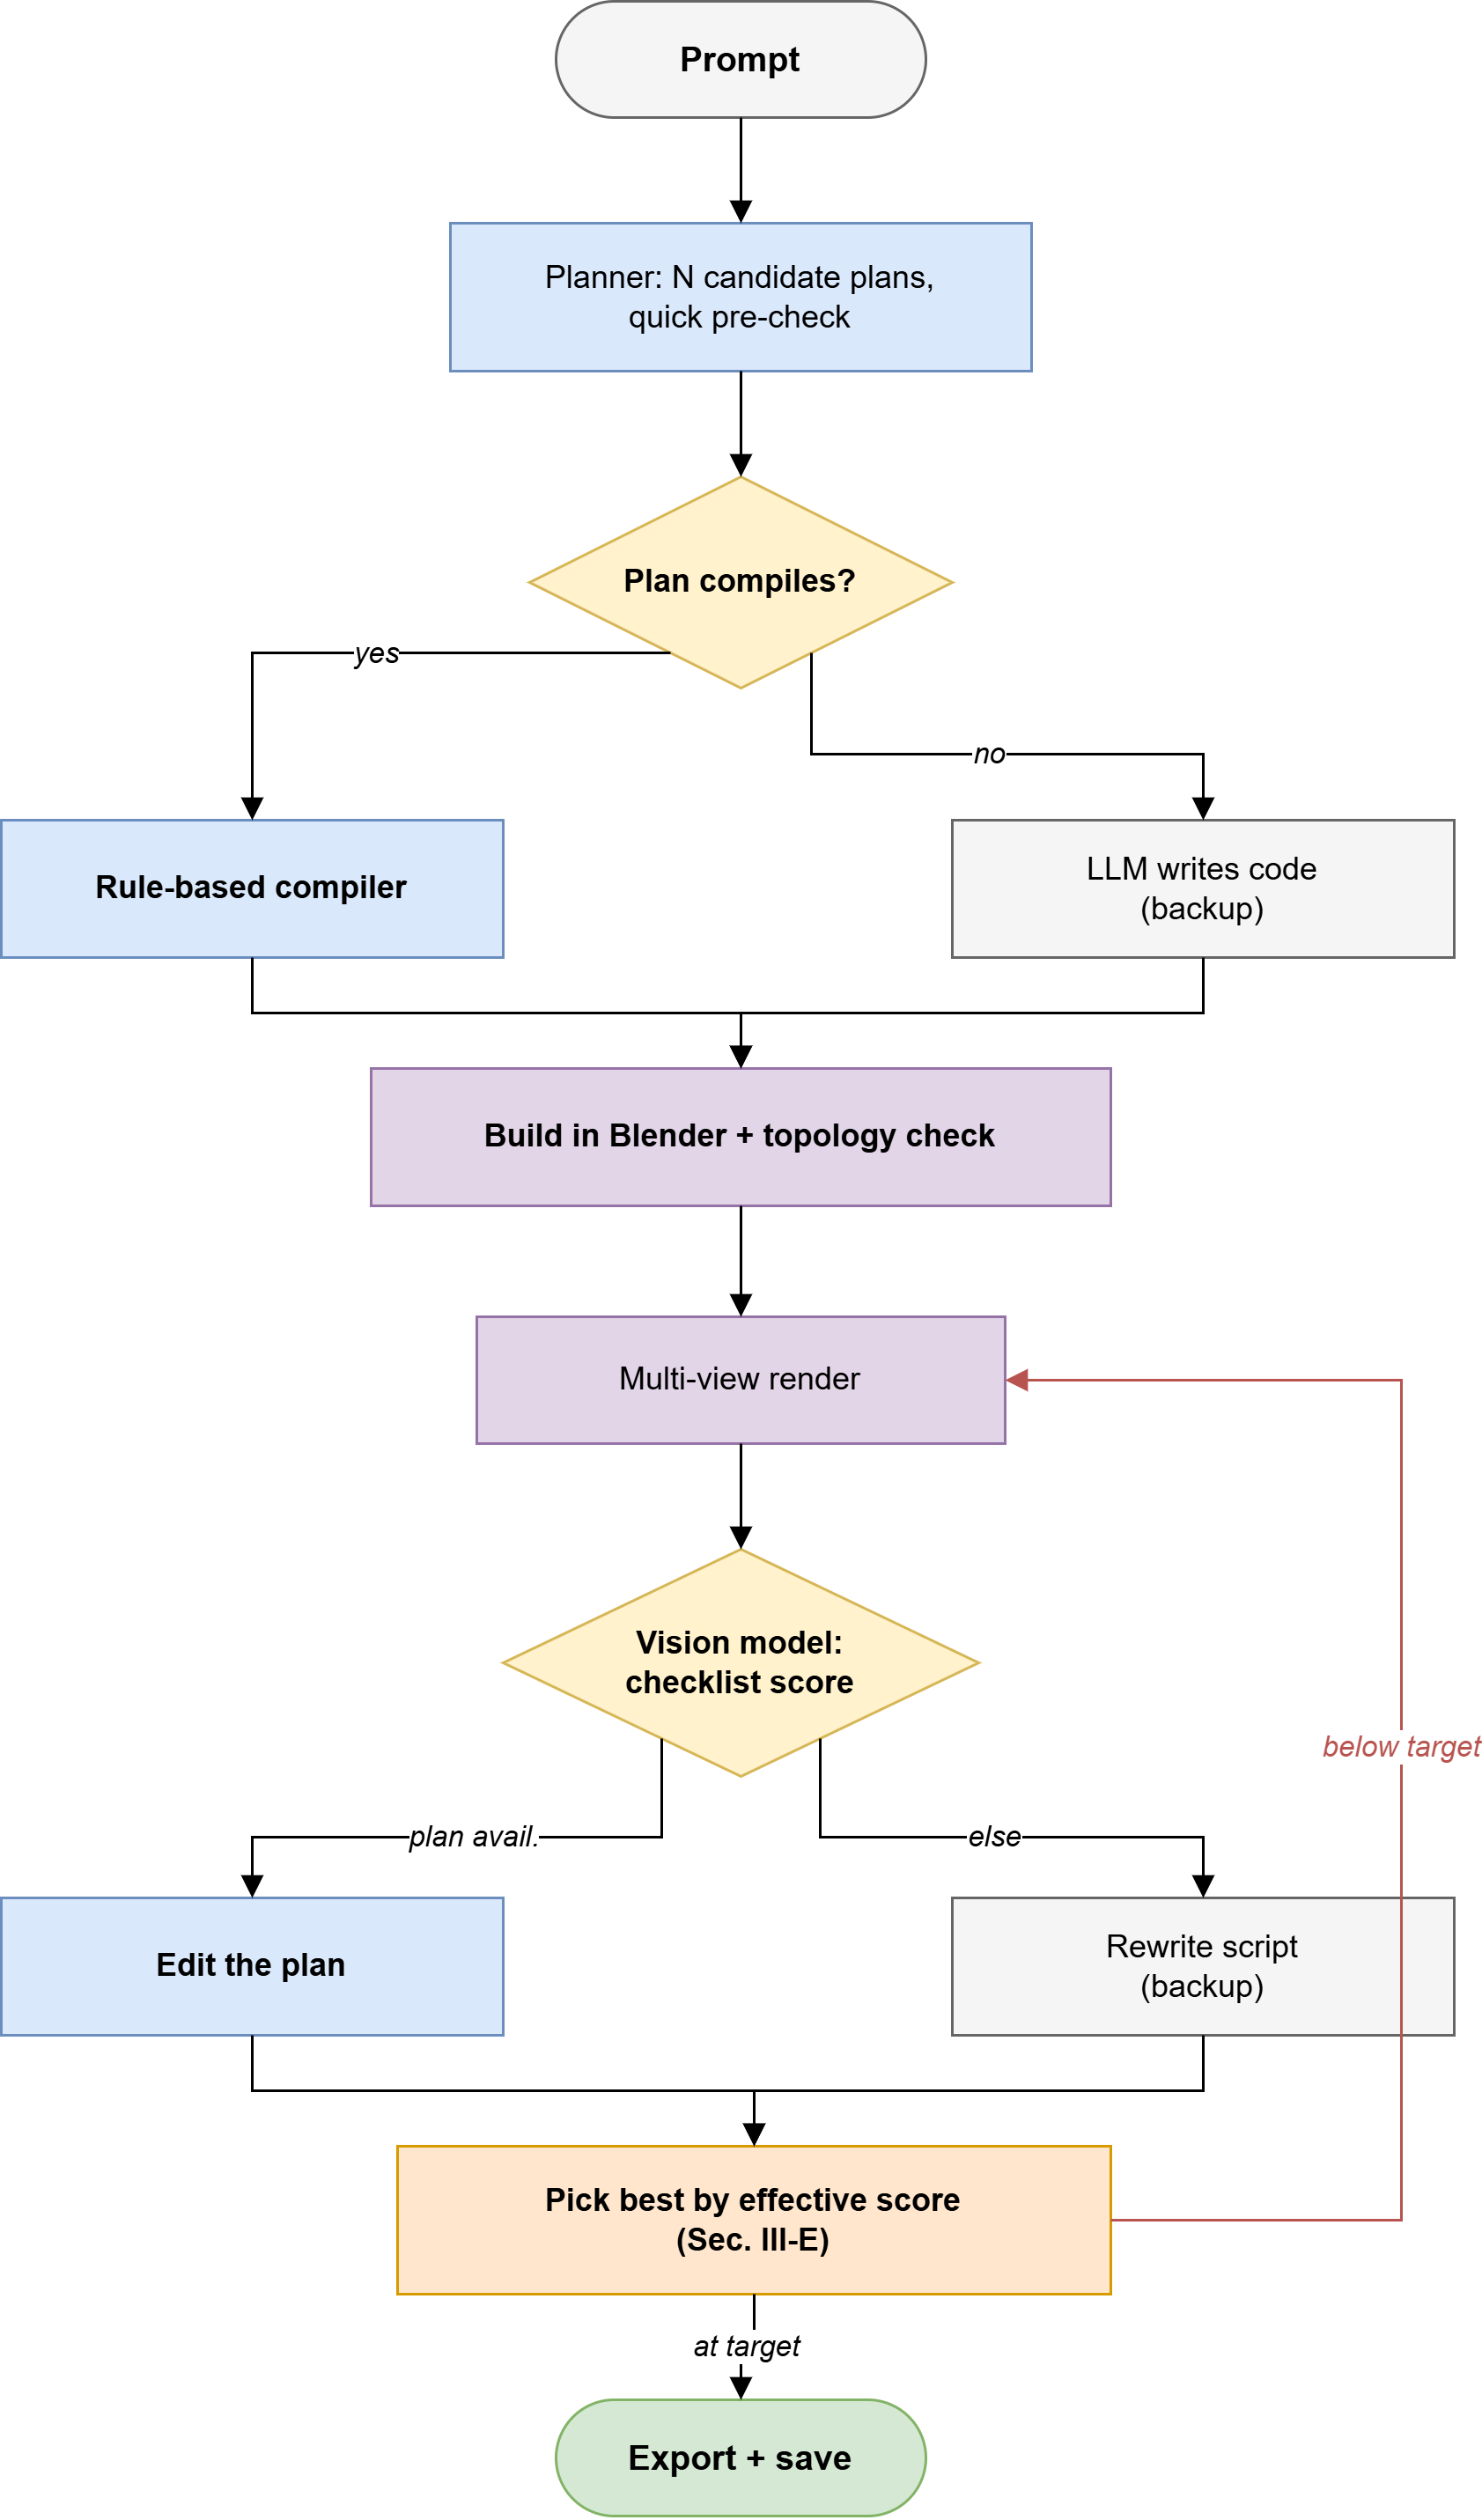
\includegraphics[width=\columnwidth]{fig1_pipeline}
\caption{The ARGUS pipeline. The compiler path (left branch) is the main path; the LLM writing code by hand (right branch) is only a backup. The repair loop after scoring also prefers editing the plan over rewriting the whole script, for the same reason.}
\label{fig:pipeline}
\end{figure}

Fig.~\ref{fig:pipeline} walks through one full run of the pipeline from start to finish. The rest of this section explains each step.

\subsection{Build Plan}
A part is a small JSON object with a name, a basic shape picked from \{\texttt{box}, \texttt{cylinder}, \texttt{sphere}, \texttt{wheel}, \texttt{bolt}, \texttt{panel}, \texttt{lathe}, \texttt{tube}, \texttt{ring}, \texttt{leaf\_card}\}, shape-specific sizes, a position, a material name, and an \texttt{attach\_to} field pointing at its parent part. Optional finishing fields are validated and clamped to safe ranges. Parts can be mirrored or repeated, and the compiler expands these operations before building. The current plan language is additive: it cannot express general subtraction such as holes, notches, or slots. This limitation is important when interpreting benchmark prompts that require internal voids.

Before building anything in Blender, the planner writes a few candidate plans at increasing randomness, has the LLM think through the object step by step first, which is similar to how step-by-step prompting has been shown to improve LLM reasoning \cite{wei2022cot}, and scores each candidate with a quick, render-free check (a simple rule about whether parts connect and sit on the ground) so a bad layout can be thrown out before Blender is even opened.

\subsection{Rule-Based Compiler}
Every shape is produced by a fixed construction routine using Blender's mesh operations. These routines are intended to produce closed primitives, but the assembled scene is still validated after placement and export. ARGUS checks for disconnected groups and other topology indicators, and may snap parts that are within a configured tolerance. A repeatable offset based on asset and part identifiers makes repeated builds deterministic for a fixed plan. The optional \texttt{fuse} operation creates a blended local surface for marked groups; it does not turn the full system into an implicit representation. These construction choices are implementation mechanisms, while the reported topology labels remain measurements of the resulting artifact.

\subsection{Materials}
The planner selects materials from a library of image-based textures and parameterized fallback materials. The evaluation counts a material as textured when the exported glTF contains a base-color texture reference; this is an artifact-level proxy and does not by itself establish material realism or semantic correctness.

\subsection{Vision-Guided Repair Loop}
The finished script, whether compiled or, on the backup path, written directly by the LLM, is run inside a hidden copy of Blender. A 2$\times$2 grid of different views is rendered and scored by a vision-language model against a checklist built straight from the plan's own part list (``is the handle visible and connected to the body,'' for every listed part-to-parent connection), instead of a free-form 1--10 rating, which our own testing found to be more reliable when using a free-tier vision model. If the score is below target, the model is first asked for a short list of JSON edits to the current plan. Only when plan-editing is not possible, because the object was made by the code-writing backup, or the edit step itself fails, does the system fall back to asking for a full script rewrite. This order, plan edit first, script rewrite second, is how ARGUS keeps each fix small and easy to check, even in the backup case where it still has to touch code.

\subsection{Selection Under Uncertainty}
\label{sec:selection}
A raw model-judged score captures some visible properties but does not directly measure exported topology or material references. In pilot debugging, we observed cases in which a visually higher-scoring candidate had fewer texture references, and a candidate with a high visual score was flagged by the topology checker. These observations motivate a candidate-selection heuristic, not a validated perceptual metric; its weights are engineering choices that require ablation and human evaluation.

So instead of the raw score, we pick the winner using an \emph{effective score}:
\begin{equation}
s_{\mathrm{eff}} = s_{\mathrm{vision}} - p(\sigma) + b(t)
\label{eq:effscore}
\end{equation}
where $\sigma$ is the topology problem level from the checker, with $p(\text{clean})=0$, $p(\text{medium})=0$, $p(\text{high})=1$, $p(\text{critical})=3$, and $b(t)=\min(0.5t,\,c)$ gives credit for $t$ textured materials up to $c=2$. The function is used only to rank candidates produced within a run. It is not bounded to the nominal 1--10 visual-score range, and its coefficients are not learned or perceptually calibrated. A new candidate replaces the current best only when its effective score is strictly higher; the component measurements and rejection reason are retained in the run log.

\subsection{Fallback Chain and Resilience}
When the compiler path is not available, script writing tries a list of backup AI providers one after another, a first try that can see images, then several text-only backups, and rotates through up to ten API keys per provider to work around rate limits. A set of hand-written backup scripts, chosen by matching keywords in the request, is used as a last resort for object types the planner cannot otherwise handle; these used to be a real source of the texture-losing bug described in Section III-E. A small, careful add-on step now matches already-downloaded photo materials onto these backup scripts' flat, made-up materials by comparing the words in their names, and it never touches a material the script already textured correctly.

\subsection{Interactive Control}
A single run can take tens of minutes. Letting the user cancel a run uses the same shared checkpoint the pipeline's own time-limit check already uses, so cancelling takes effect at the next natural break in the loop, and the pipeline still finishes exporting and checking whatever was already built, instead of just killing the process outright.

\section{Implementation}
The main program is a Python process that drives a hidden copy of Blender 5.0 through a subprocess, and exports GLB, FBX, and a native \texttt{.blend} file. The desktop app is built with Tauri and React, talking to a FastAPI backend that sends pipeline progress as a stream of typed events, stage changes, key/value updates, scores, and the final result, replacing an older setup where two separate parts of the app each tried to read the same plain-text console output with their own pattern-matching code, a fragile setup this version removes completely instead of patching around. The test suite (Section V) runs each (prompt, setting) pair as its own separate process, since the output folder is set once when the Python module first loads, so testing each pair on its own needs a brand-new process; the numbers are then computed directly from the exported glTF file's own data (triangle count, vertex count, material count, embedded image count) instead of by rendering again, so re-checking a finished set of results costs nothing and can never disagree with itself between runs.

\section{Evaluation}
\label{sec:eval}

\subsection{Test Set}
We built a 30-prompt test set split into three hard-surface difficulty levels: \emph{simple}, \emph{moderate}, and \emph{complex}. The benchmark is intentionally domain-specific and is not a general text-to-3D benchmark. This paper reports a pilot run of 5 prompts per level (15 total) using the system's normal settings. The remaining prompts and comparison conditions are part of the public harness but are not treated as completed experiments here.

\subsection{Metrics}
Artifact metrics are read from the exported glTF: triangle count, vertex count, mesh count, material count, textured-material count, and embedded image count. A material is counted as textured when its glTF material contains a base-color texture reference. The topology level and ground-contact flag come from the in-process checker. Visual quality is a model-judged checklist score and has not been validated against human ratings. We also report taper-option uptake as an implementation diagnostic; it is not an outcome-quality metric.

\subsection{Results}
Table~\ref{tab:overall} summarizes the 15-prompt pilot; Table~\ref{tab:perasset} lists every reported result. All 15 prompts produced an exported artifact under the evaluation harness's completion criterion. This should not be read as evidence that all prompts were semantically or perceptually successful. No artifact was classified as \texttt{critical}; 13/15 were classified as clean and 13/15 contained at least one base-color texture reference. The mean raw visual score was 6.67/10. The heuristic effective score reached 8 or more for 9/15 cases, but this threshold is an internal selection threshold rather than a validated quality standard. All aggregate values are computed by the repository's reporting code from the deduplicated final record for each condition/prompt pair.

\begin{table}[t]
\centering
\caption{Pilot test run summary (15 prompts, normal settings)}
\label{tab:overall}
\begin{tabular}{lccc}
\toprule
Metric & Simple & Moderate & Complex \\
\midrule
$n$ & 5 & 5 & 5 \\
Build completion & 100\% & 100\% & 100\% \\
Mean visual score & 6.4 & \textbf{7.6} & 6.0 \\
$\geq$7/10 & 60\% & 80\% & 40\% \\
Clean topology & 80\% & \textbf{100\%} & 80\% \\
Critical topology & 0\% & 0\% & 0\% \\
Textured & \textbf{100\%} & 60\% & \textbf{100\%} \\
Mean triangles & 3{,}565 & 20{,}157 & 63{,}856 \\
Mean time (s) & 599 & 736 & 1{,}027 \\
\bottomrule
\end{tabular}
\end{table}

\begin{table*}[t]
\centering
\caption{Result for every asset in the pilot test run}
\label{tab:perasset}
\small
\begin{tabular}{lllccccc}
\toprule
ID & Level & Prompt & Score & Topology & Textures & Triangles & Time (s) \\
\midrule
b01 & simple   & a wooden crate                 & 7 & high  & 5  & 7{,}600   & 669 \\
b02 & simple   & a steel oil drum               & 7 & clean & 1  & 5{,}624   & 897 \\
b03 & simple   & a traffic cone                 & 5 & clean & 4  & 1{,}276   & 413 \\
b04 & simple   & a cardboard shipping box       & 6 & clean & 9  & 1{,}820   & 678 \\
b05 & simple   & a concrete cinder block        & 7 & clean & 1  & 1{,}504   & 335 \\
b09 & moderate & a cast iron fire hydrant       & 8 & clean & 0  & 18{,}672  & 242 \\
b10 & moderate & a rustic park bench            & 5 & clean & 3  & 5{,}952   & 1{,}334 \\
b11 & moderate & a fire extinguisher            & 8 & clean & 0  & 6{,}748   & 1{,}422 \\
b12 & moderate & a street lamp post             & 8 & clean & 17 & 4{,}216   & 387 \\
b13 & moderate & a wooden step stool            & \textbf{9} & clean & 1  & 65{,}196  & 294 \\
b21 & complex  & a steam locomotive engine      & 6 & high  & 25 & 21{,}096  & 766 \\
b22 & complex  & a wooden windmill              & 8 & clean & 5  & 4{,}996   & 776 \\
b23 & complex  & an anglepoise desk lamp        & 7 & clean & 14 & 3{,}560   & 1{,}641 \\
b24 & complex  & a vintage gas pump             & \textbf{3} & clean & 19 & \textbf{281{,}182} & 938 \\
b25 & complex  & a wheelbarrow                  & 6 & clean & 14 & 8{,}444   & 1{,}016 \\
\bottomrule
\end{tabular}
\end{table*}

\begin{figure}[t]
\centering
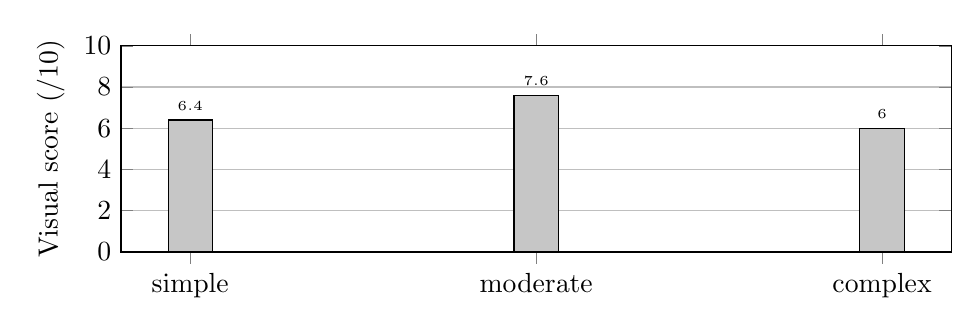
\begin{tikzpicture}
\begin{axis}[
  ybar, width=\columnwidth, height=4.2cm,
  ylabel={Visual score (/10)}, ymin=0, ymax=10,
  symbolic x coords={simple,moderate,complex},
  xtick=data, nodes near coords, nodes near coords style={font=\tiny},
  bar width=16pt, ymajorgrids, axis on top=false,
]
\addplot[fill=gray!45] coordinates {(simple,6.4) (moderate,7.6) (complex,6.0)};
\end{axis}
\end{tikzpicture}
\caption{Average model-judged visual score by difficulty level in the pilot. The moderate level exceeds the simple level in this sample, although the comparison is confounded by reference assets and the small sample size.}
\label{fig:tierbar}
\end{figure}

\subsection{Qualitative Analysis}
\label{sec:qualitative}
Two results in Table~\ref{tab:perasset} are worth a closer look.

\emph{Moderate exceeds simple in the pilot.} Fig.~\ref{fig:tierbar} shows the moderate level scoring higher on average (7.6) than the simple level (6.4). Four of the five moderate prompts have a hand-checked reference in the shape library, so the observed difference is confounded by reference availability and should be treated as a hypothesis for a larger controlled study, not as a difficulty effect.

\emph{The gas-pump outlier.} b24 scored 3/10, the lowest score in the whole test run, even though it had clean topology and 19 real textured materials, at 281{,}182 triangles: about $4.3\times$ more than the next-highest object in the entire run (b13, at 65{,}196). A low score next to clean topology and full texturing does not match the usual failure pattern this paper focuses on in Section III-E, a high score hiding a real problem. We think this is instead a separate, unrelated geometry bug, most likely a modifier stack that ran out of control, or an unlimited part-repeating step tied to how many parts this specific prompt asked for. Our current numbers can flag this case, since the triangle count is an obvious outlier, but cannot explain it. We are reporting it honestly instead of leaving it out.

Fig.~\ref{fig:qualgrid} turns the topology numbers in Table~\ref{tab:overall} into something you can actually look at, showing six objects from the test run in both their finished, rendered form and as raw wireframe geometry.

\begin{figure*}[t]
\centering
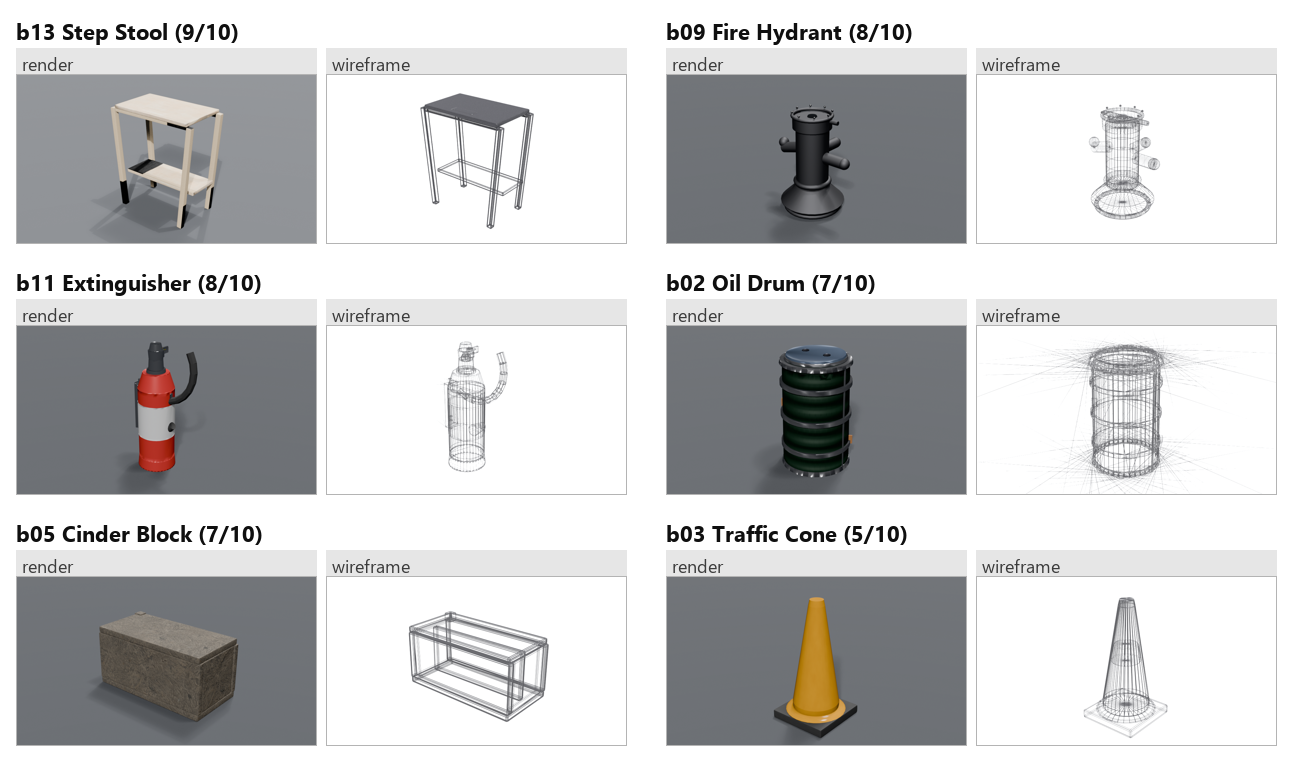
\includegraphics[width=0.92\textwidth]{fig3_qualitative_grid}
\caption{Render and wireframe pairs, from the same camera angle, for six objects from the test run: the highest-scoring result at each difficulty level plus three more objects with clean topology. The wireframes are real renders of each object's exported geometry, not drawings made to illustrate the idea.}
\label{fig:qualgrid}
\end{figure*}

\subsection{An Infrastructure Finding}
\label{sec:dns}
During collection, 12 of the 30 raw attempts behind the 15 reported cells recorded a DNS lookup error. Each affected cell later recovered on retry, so the reported pilot uses the final successful record for each prompt. The incident demonstrates why network failures must be tracked separately from generation quality; the precise provider-retirement timeline is environment-specific and is not treated as a research result.

The measurement lesson is that a network signature should not automatically invalidate a completed asset. The evaluator therefore requires corroboration: a run counts as an environment failure only when the signature appears and no scored asset is produced. This rule keeps the attempt history available for audit while preventing fallback-chain noise from being mistaken for a quality failure.

\section{Threats to Validity and Limitations}
\label{sec:limits}
We are putting these limits up front instead of burying them at the end, because several of them change how the results above should be read.

\begin{itemize}
\item \textbf{No causal ablation study.} The harness supports multiple on/off conditions, but the pilot does not establish which component causes the observed behavior. The compiler, repair loop, candidate count, scoring heuristic, and other settings must be isolated in a controlled study.
\item \textbf{No external baseline.} The pilot has not been compared with a feed-forward generator or an LLM-code system under matched prompts and metrics, so no superiority claim is warranted.
\item \textbf{One noisy judge, no human study.} The only visual-quality judge is a vision-language model. Its repeatability and agreement with human ratings have not been measured, so the visual scores should be interpreted as model outputs rather than ground-truth quality.
\item \textbf{Small sample size.} Fifteen pilot results are insufficient for strong statistical conclusions; tier differences and outliers are exploratory observations.
\item \textbf{Limited scope.} The test set and the plan format are built for still, hard-surface, mostly non-living objects. Living or organic shapes, characters, and full scenes with multiple objects are simply out of scope by design, not something we tried and failed at.
\item \textbf{No cutting holes.} The plan format can only add material, aside from the one optional fuse tool; holes, notches, and slots, which are common on real hard-surface objects, cannot be described yet.
\item \textbf{Environment dependence.} All pilot tests used one computer and free-tier API limits; timings, retries, and provider behavior may differ on other hardware or services.
\end{itemize}

\section{Future Work}
The next study should run the supported ablations across all 30 prompts, compare ARGUS with at least one external text-to-3D baseline and one direct-code baseline, and collect repeated model judgments plus human ratings. The plan language should also gain explicit subtraction operations for holes, notches, and slots. A signed-distance-field method may support a wider range of joints, but it should be evaluated as an extension rather than assumed to improve the current polygon-based path.

\section{Conclusion}
ARGUS separates high-level spatial planning from low-level scene construction through a structured plan and a deterministic compiler. The pilot shows that this representation can be executed, exported, and measured across a small hard-surface prompt set, while also exposing the limitations of model-judged visual scores and heuristic candidate selection. The results are a systems characterization, not evidence of comparative superiority: causal ablations, external baselines, and human evaluation remain necessary before stronger performance claims can be made.

\section*{Acknowledgment}
The author thanks Mr.\ Anmol Pandey, Assistant Professor, Department of Computer Engineering, Sikkim Institute of Science and Technology, for guiding the earlier version of this system \cite{dahal2026thesis} that this paper builds on.

\bibliographystyle{IEEEtran}
\bibliography{references}

\end{document}
